\section{Video Player}
\subsection{Ziel}
In einem ersten Schritt, noch vor der Realisierung des Fahrsimulator wird ein Video-Player ralisiert. Das Ziel des Video-Players ist es eine Verbindung zwischen dem Cockpit und unserem Programm herzustellen und diese zu Testen. Bei der Betätigung des Gaspedals im Cockpit soll das aufgenommene Video schneller abgespielt werden. Bei der Betätigung des Bremspedals dementsprechend langsamer. Der Video-Player soll so gegliedert werden, damit Komponenten davon auch im Fahrsimulator wiederverwendet werden können. Zudem ist die Darstellung einer Tunneleinfahrt mit den richtigen Lichtverhältnissen in einer 3D-Umgebung sehr schwierig. Eine gute Alternative bietet ein aufgenommenes Video einer Tunneleinfahrt. Die ETH-Zürich besitzt bereits Videos die sich dafür eigenen. Um Experimente mit diesen Videos durchführen zu können, müssen Manipulationen die der Proband im Cockpit mach mit dem entsprechenden Zeitpunkt im Video abgespeichert werden. Dies dient zur späteren Auswertung der Experimente. 

\subsection{Systembeschreibung}

% Bild für Systembeschreibung des Video Players
\begin{figure}[H]
\centering 
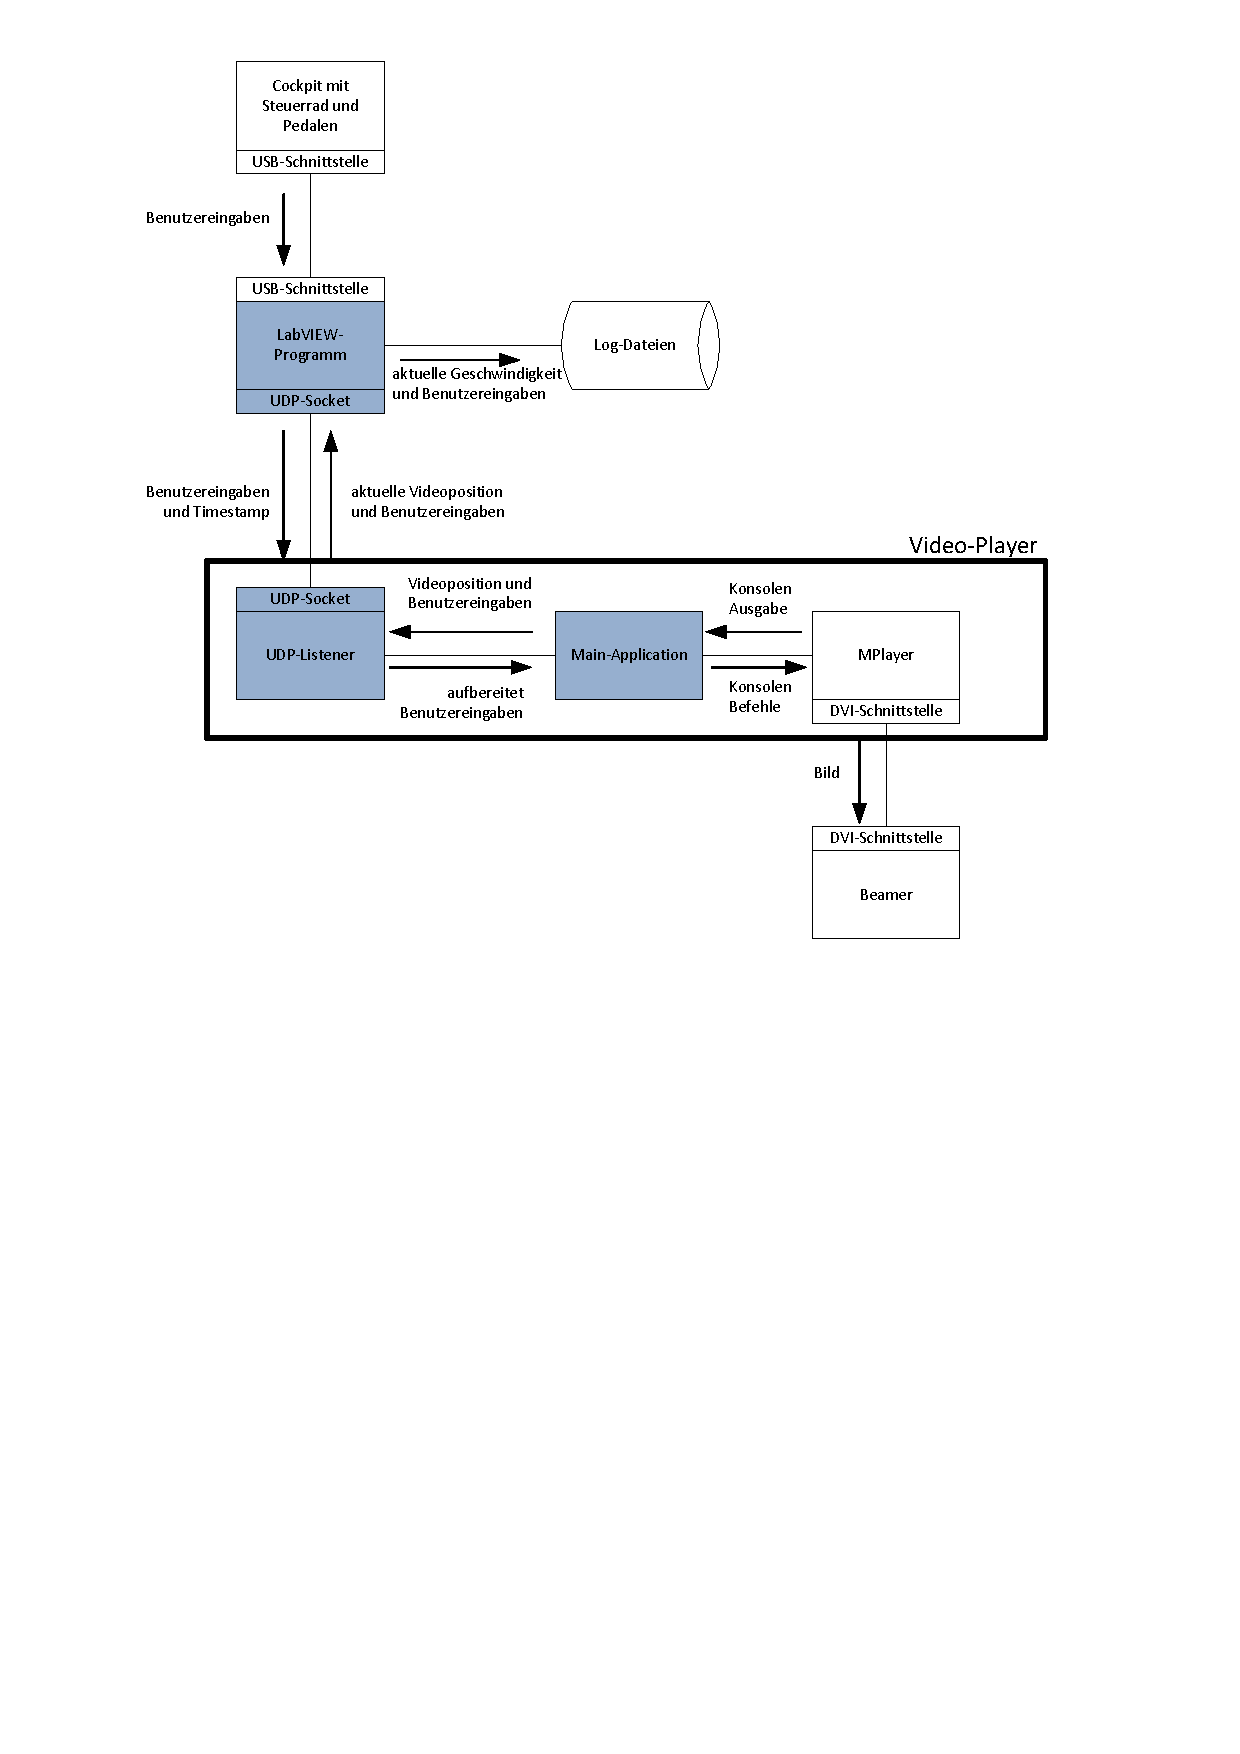
\includegraphics{src/Systembeschreibung_VideoPlayer.pdf}
\caption{Systembeschreibung Video-Player} % Titel der Grafik
\label{Systembeschreibung Video-Player} % Labelname
\end{figure}
Um einzelne Komponenten des Video-Player wiederverwenden zu können, wird das System möglichst gleich wie das des Fahrsimulators aufgebaut. Dieser Aufbau wird anhand der Abbildung \ref{Systembeschreibung Video-Player} illustriert.  Die blau markierten Komponenten werden im Rahmen des Video-Players entwickelt. Alle überigen sind bereits vorbestehend. \\
Die LabVIEW-Komponente in der Abbildung \ref{Systembeschreibung Video-Player} liest bereits die Eingaben die der Proband im Cockpit mach ein. Diese wird mit einem UDP-Socket erweitert um die Eingaben des Probanden an den Video-Player weiterzuleiten. Die UPD-Packete sollen vom UDP-Listener gelesen werden und die in ihnen enthaltenen Parameter gespeichert werden. Das Hauptprogramm soll auf die gespeicherten Parameter Zugriff haben. Aufgrund der Parameter soll das Hauptprogramm die Abspielgeschwindigkeit des Videos manipulieren, das mit einem Programm abgespielt wird. Durch mehere Versuche hat sich gezeigt das sich der MPlayer am besten für solch eine Aufgabe eignet. Dies wird in der Ralisierung ausführlich dokumentiert. Der MPlayer soll die Position im Video an das Hauptprogramm übergeben können. Das Hauptprogramm soll diese Information der Video-Position mit den getätigten Eingaben des Probanden ergänzen und dies an den UDP-Listener übergeben. Über den UDP-Sockes sollen die Daten an das LabVIEW-Programm gesendet werden. Dort muss zusätzlich ein Port eingerichtet werden um UDP-Packete zu empfangen. 

Eine wird erweitert wie in Kapitel 3.1 dokumentiert. 


Die LabVIEW-Komponente in der Abbildung \ref{Systembeschreibung Video-Player} liest bereits die Eingaben die der Proband im Cockpit mach ein. Dieses muss nun so erweitert werden, dass diese über einen UDP-Socket an das Programm übertragen werden. Zusätzlich muss im LabVIEW ein UDP-Port eingerichtet werden, der verwendet werden kann, um UDP-Packete zu empfangen. Dieser wird benötigt um Daten die von unserem Programm gesendet werden in ein Log-File zu schreiben.
Die Parameter werden vom vom UDP-Listener gespeichert und vom Hauptprogramm abgefragt. Aufgrund der Parameter wird dann die Geschwindigkeit des Videos manipuliert. Für das Abspielen des Videos wird der mPlayer verwendet. Die Befehle für den mPlayer können von unserem Programm über die Komandozeile abgesetzt werden. Ausgaben vom mPlayer  werden ebenfalls über die Komandozeile den Standartausgang der Konsole übergeben. 

\subsection{Realisierung}
In einem bestehendem LabVIEW-Programm werden bereits alle Eingaben, die im Cockpit gemacht werden können, eingelesen. Nun muss dieses Programm nur noch mit einem UDP-Port erweitert werden, damit es die Parameter, die unser Video-Player benötigt, senden kann. Diese Daten sind im Video-Player vor allem die betätigung von Gas- und Bremspedal. Diese beiden Pedalen werden in einem Koordinatensystem wie in Abbildung \ref{Koordinatensystem2} auf der y-Achse abgebildet. Die positive y-Richtung verifiziert das Gas und die negative y-Richtung das Bremspedal. Die intensität beider Pedalen wird durch 32767 bzw. 32768 ganzzahlige Werte identifiziert. Wenn also keins der beiden Pedalen gedrückt ist, wird dies durch den y-Wert 0 verifiziert. Ein voll gedrücktes Gaspedal entspricht dem y-Wert 32767 und dementsprechend ein voll gedrücktes Bremspedal dem Wert -32768. Der x-Wert im Koordinatensystem verifiziert den Einschlagswinkel des Steuerrades. Ist das Steuerrad in der neutralen Stellung, entspricht dies dem x-Wert null. Wenn das Steuerrad vollständig nach rechts eingeschlagen ist, wird dies durch den positiven x-Wert 32767 identifiziert. Dementsprchend wird ein vollständiger Einschlag nach links durch den negiativen x-Wert -32768 identifiziert. \\

\begin{figure}[H]
\centering 
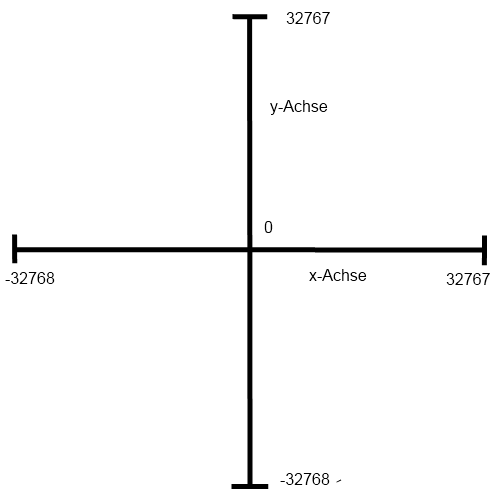
\includegraphics[scale=0.5]{src/koordinatensystem.png}
\caption{Koordinatensystem} % Titel der Grafik
\label{Koordinatensystem2} % Labelname
\end{figure}

Diese beiden Werte werden im LabVIEW-Programm in ein UDP-Packet verpackt und über das Netzwerk gesendet. Der UDP-Listener empfängt diese Packete und speichert die x und y-Werte separat ab. Das Hauptprogramm greift auf diese Werte zu, interpretiert diese und Steuert das Video.\\
Der Video Player wird in einem eigenen Prozess gestartet. 
% Code
%sprintf(arguments, " --extraintf telnet --telnet-port %d --telnet-password %s", vlcPort, vlcPassword);
%CreateProcessA(vlcExe, arguments, 0, 0, FALSE, 0, 0, 0, LPSTARTUPINFOA(&si), &pi);
%Code ende
Die erste Zeile speichert alle Argumente in der Variabel "arguments". Durch die mitgegebenen Argumente wird der Video Player mit einem extra Telnetinterface gestartet.  Das Telnetinterface hört auf den angegebenen Port. In der zweiten Zeile wird der Prozess erstellt und in diesem Prozess wird der Video Player ausgeführt. 
Nun können Manipulationsbefehle über den "send" Befehl an den mPlayer geschickt werden. Hier ein Beispiel eines solchen Befehls.
%Code
%send(socketId, message, strlen(message)
%CodeEnde
Der send-Befehl verlangt eine Socket-Id, die Nachricht,  in unserem Fall den Befehl, und die Länge der Nachricht. Das Hauptprogramm liest nun aus dem UDP-Listener den y-Wert der empfangenen Packete aus. Liegt dieser Wert über 20000 ist das Gaspedal mindestens zu zwei drittel gedrückt. Dann sendet das Hauptprogramm über die Telnetverbindung den Befehl an den Video Player die Geschwindigketi des Videos zu erhöhen. Fall der Wert unter -20000 liegt, ist das Bremspedal mindestens zu zwei drittel gedrückt. Das Hauptprogramm veranlasst den Videoplayer die Geschwindigkeit des Videos u reduzieren. 